\section{Introducci�n}

\subsection{Motivaci�n}
% \noindent
Actualmente es posible escribir en dispositivos electr�nicos, sobre todo con la llegada de las Tablet PC, pizarras el�ctricas, celulares touch-screen y las pantallas t�ctiles. Tambi�n cabe destacar algunos e-Readers que permiten la escritura, convirti�ndose en \textit{papel electr�nico}. La escritura se realiza generalmente con un \textit{stylus} (l�piz), abriendo la puerta a nuevas interacciones m�s all� del teclado y mouse. En la figura \ref{tabletas}, puede apreciarse una variedad de dispositivos que permiten la escritura con l�piz.
\begin{figure}[!htbp]
 \centering
 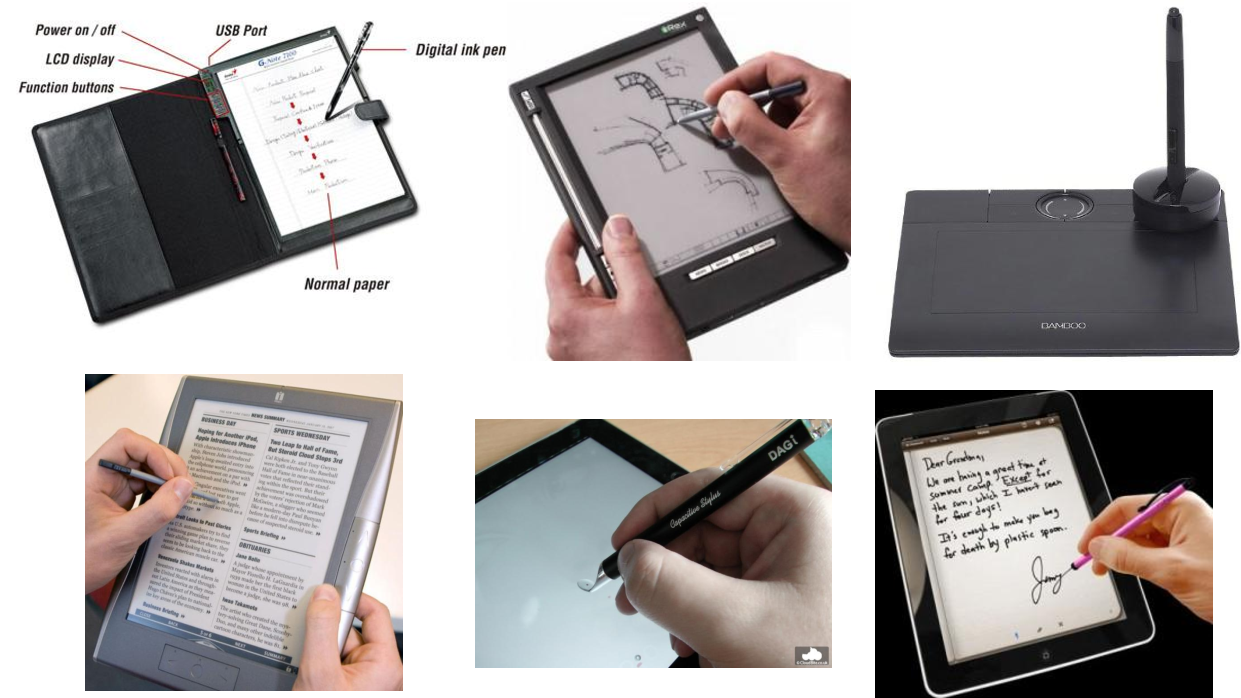
\includegraphics[scale=0.65]{imagen/tabletas.pdf}
 \caption{Tabletas}
 \label{tabletas}
\end{figure}

A pesar de que exista una variedad importante de tales dispositivos, no hay todav�a una aplicaci�n sobresaliente de reconocimiento para ellos. El usuario ve al \textit{stylus} como un mouse sofisticado, sin que se logre una mejora significativa en la productividad al no explotar la potencialidad del mismo. Un buen sistema de reconocimiento de escritura (\textit{handwriting recognition}\footnote{Muchos t�rminos utilizados aqu� se dejan intencionalmente en ingl�s, facilitando la b�squeda de contenido para tales t�rminos.}) podr�a permitir al usuario una mejor experiencia con respecto al papel y l�piz tradicional, permiti�ndole obtener resultados inmediatos a partir de su escritura, como ser resultados matem�ticos.



\subsection{Organizaci�n del trabajo}
En la secci�n \ref{sec:Conceptos_Generales} se introducen los concepto generales de reconocimiento de escritura; la secci�n \ref{fundamentos}, se introducen los fundamentos te�rico en lo que se basa el trabajo; secci�n \ref{feature_extraction}, se explica la extracci�n de caracter�sticas; secci�n \ref{clasificacion}, se comentan los m�todos de clasificaci�n utilizados; secci�n \ref{sec:resultados}, se comparan todos los m�todos; secci�n \ref{sec:aplicaciones}; se provee una visi�n futura de las posibles aplicaciones de los m�todos explicados; y por �ltimo, secci�n \ref{sec:conclusion}, la conclusi�n.
